\chapter{Widefield image synthesis}
%%%%%%%%%%%%%%%%%%%%%%%%%%%%%%%%%%%%%%%%%%%%%%%%%%%%%%%%%%%%%%%%%%%%%%%%%%%%%%%%%%%%%%%%%%% MORE ABOUT THE CORRELATOR ONCE WE DISCUSSED FOURIER THEORY

% It is worthwhile to note that the correlation, delay and phase compensations can also be done in the fourier domain, and in the case of delay compensation this approach makes fractional delay compensation feasible (see Taylor et al. \cite{taylor1999synthesis}). These correlators are effectively 
% known as \textit{FX} correlators. If these power spectra are of high time resolution it is possible to perform surveys focussed on transient detection. Modern arrays such as LOFAR, KAT-7 and MeerKAT (currently under construction) have the capability to perform these searches through
% special \textit{beamforming} modes which may be run concurrently with imaging modes. See Stappers et al. \cite{stappers2011observing} for details on pulsar observation with LOFAR. In this thesis, however, we will focus solely on the imaging pipeline which is discussed in the next section.
% 
% In the previous section the response, $r$, of a complex correlator was described. The \textit{visibility} is an unnormalized measure of the coherence of an electric field, and is very closely related to the correlator response to the planar wave fronts emitted
% by a source. The magnitude of this coherence has dimensions of flux density as described earlier. The Radio Interferometric Measurement Equation relates between these visibilities and the projection of the source onto the celestial sphere. This projection and measurement
% process is illustracted in figure~\ref{fig_uvw_lmn}. Without loss of generality when extended to the different polarization terms, the relation between the measured visibilities and the image can be defined as:
% \begin{equation}
%  \label{eqn_visibility}
%  \begin{split}
%   V(u,v,w) &:= \int_{\vec{s}}{A(\vec{s})I(\vec{s})\cos{\frac{2\pi\vec{b}\cdot(\vec{s}-\vec{s_0})}{\lambda}}d\Omega}\\
% 	   &= \int_{-\infty}^\infty{\int_{-\infty}^\infty{A(l,m)I(l,m)e^{-2\pi i[ul+vm+w(n-1)]} \frac{dldm}{\sqrt{1-l^2-m^2}}}}\\
% 	   &= \int_{-\infty}^\infty{\int_{-\infty}^\infty{A(l,m)I(l,m)e^{-2\pi i[ul+vm+w(\sqrt{1-l^2-m^2}-1)]} \frac{dldm}{\sqrt{1-l^2-m^2}}}}
%  \end{split}
% \end{equation}
% 
% \begin{figure}[h]
%  \begin{mdframed}
%  \centering
%  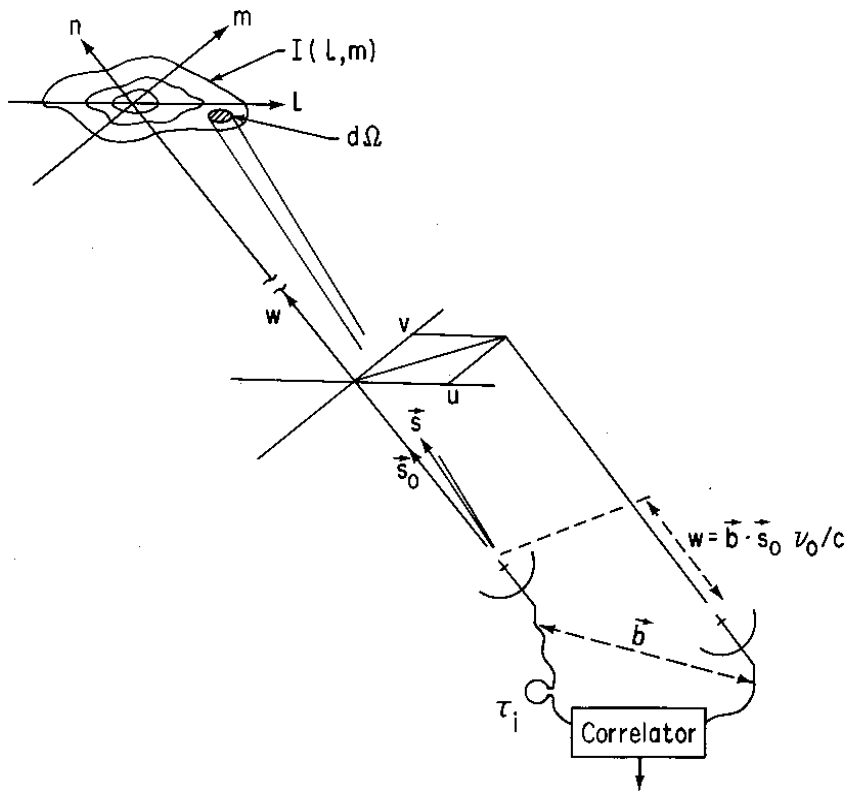
\includegraphics[width=0.5\textwidth]{images/lmn_uvw.png}
%  \caption[The relation between image space and visibilities]{The relation between the measured spatial coherence function and the source on the unit ``celestial'' sphere, emitting planar waves of radiation \cite{taylor1999synthesis}.}
%   \label{fig_uvw_lmn}
%  \end{mdframed}
% \end{figure}
% 
% When the field of view being observed is sufficiently small, $n$ is close to unity and the term $w(n-1) = 0$. Similarly, if the all the antenna are at equal height (\textit{co-planar}) $w=0$ and the term disappears as well. Under 
% these circumstances equation~\ref{eqn_visibility} is the two dimensional fourier transform of the image. In reality the image is not only affected by the effective area of the comprising elements in the interferometer, but is 
% subject to incomplete sampling, direction-independent antenna gains, as well as directional effects, such as ionospheric and tropospheric conditions. 
% 
% Each observation will typically extend over a prolonged period of time (over many hours for instance) and collect a large number of visibilities, typically over a large number of channels. As the earth rotates each baseline sweeps out
% eliptical paths in u,v space, sampling the coherence function at regular intervals. As the number of antennae in the array is increased the number of measured visibilities grow quadratically, since the number of possible baselines between 
% antennae is given as $\frac{n(n-1)}{2}+n$. Adding a small number of antennae to the array can therefore effectively improve the uv coverage. By adding more visibilities in fourier space the quality of the synthesized 
% image is improved, because the effects of the limited sampling can be more effectively removed from the produced image as is explained in the section on convolutional gridding.
% 
% The uniform and wide coverage of the entire u,v space (the size of which is determined by the required angular resolution), can normally be attained using only east-west baselines, except at very low declanations (less than about $30^o$) at the horizon. At low declanations baselines 
% with a component sufficiently parallel to the Earths axis (non East-West) are needed. Such a two dimensional array have baseline components which don't remain co-planar over long observations and require the l and m components being small enough to 
% ensure $(\sqrt{1 - l^2 - m^2} - 1)w \approx 0$. See figure~\ref{fig_VLBA_uv} for an illustration of the uv-coverage attained by the VLBA array. The spacing in such an East-West array is of high importance
% in ensuring the uniform sampling of the u,v space. Spacing the antennas uniformly for instance will result in many redundant coverages by the shorter baselines. Other designs include movable
% antennae provide greater flexibility and can cover more baselines. For two dimensional arrays reducing redundancy becomes even more challenging as eluded to in Synthesis Imaging II \cite[Lecture 2]{taylor1999synthesis}.
% 
% \begin{figure}[h]
%  \begin{mdframed}
%  \centering
%  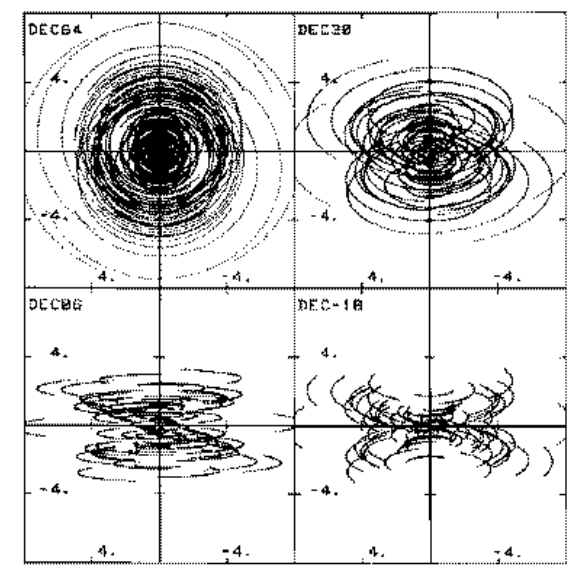
\includegraphics[width=0.5\textwidth]{images/eliptical_sampling.png}
%  \caption[VLBA uv-coverage]{The sampling patterns of the ten antennae of the VLBA at 4 different declanations. The best coverage is attained at greater declanations}
%   \label{fig_VLBA_uv}
%  \end{mdframed}
% \end{figure}
 
%%%%%%%%%%%%%%%%%%%%%%%%%%%%%%%%%%%%%%%%%%%%%%%%%%%%%%%%%%%%%%% CORRECTING THE RIME TERMS %%%%%%%%%%%%%%%%%%%%%%%%%%%%%%%%%%%%%%%%%%%%%%%%%%%%%%%%%%%%%%%%%%%%%%%% 
 
%  Correcting for known time-uniform directional effects can be achieved through either a facet-based polyhedron approach or through AW-projection. Using a image-space facet-based approach these directional
%  effects are locally-invariant and are corrected for over small portions of the final image, by multiplying with the appropriate inverse Jones matricies. In AW-projection these effects can be corrected for by convolving with
%  transposed Jones matricies, and this can be integrated to either the convolutional gridding (reverse Fast Fourier Transform) or degridding (forward Fast Fourier Transform) strategies which will be discussed 
%  in the next chapter \cite{2011A&A...527A.107S}. Both facet-based and AW-projection approaches will be discussed further in the chapter on non-coplanar wide-field imaging.
%  
%  Another approach is to subtract the directionally dependent effects directly from the observed visibilities, before correcting for the directional independent effects at the model
%  subtraction phase. Such an approach corrects these effects individually per model source and is equivalent to evaluating equation~\ref{eqn_RIME} for a set of discrete sources. These
%  analytical approaches are computationally prohibative, when compared to the convolution gridding approaches, coupled with either W-projection-based or faceting techniques, although 
%  it has the advantage of being much more accurate \cite{2011A&A...527A.107S}.
 
% \subsubsection{Self-calibration}
%  The lack of strong calibrators near observed areas, and the requirements placed on the properties of these calibrations, makes the process of calibrating the rapidly varying 
%  directional effects within the atmosphere a very hard problem. By allowing the individual element gains to be free parameters forms the basis of self-calibration. 
% 
%  Self-calibration imposes some restrictions: information about the absolute position, structure and intensity of an observed source is traded
%  for improved signal-to-noise ratios. It should be noted that these minimization approaches cannot completely replace the methods of source and polarization calibration mentioned earlier. 
%  The effect of these issues are normally incorporated as explicit Jones terms in the model, such as the one mentioned earlier. These effects are greatly reduced by adding additional 
%  antennae to the array. The self-calibration problem can be viewed as iteratively improving an initial model by correcting the effects of gain on sky brightness through algorithms such as the Maximum Entropy Method
%  and the CLEAN algorithm. The specification of the initial model does not necessarily have to be very accurate for CLEAN to converge at some point: it may simply 
%  consist of point sources for relatively simple images. Convergence is, however, not guarenteed.
% 
%  The H\"ogbom CLEAN algorithm locates (and keeps a list of) the brightest sources in an image in an iterative cycle, subtracting the Point Spread Function from each source until some 
%  thresholding condition is met. The remaining image is termed the residuals. After convolving the found point sources with elliptical function fitted over the Point Spread Function, 
%  the residuals are added to the convolved image, forming the final ''clean" image. Many other variations on the algorithm exist, bringing with them improvements in execution speed and 
%  stability.
% 
%  While CLEAN provides a procedural approach to deconvolution, the Maximum Entropy Method selects an image that fits the data to within a specified noise level, and is not procedural.
%  The method essentially limits the range of pixel values and focusses these ranges around bright objects. Though CLEAN is usually much faster on smaller simple images, it is prohibatively slow 
%  on large complex images. Under these conditions the Maximum Entropy Method is outright faster.
% 
%  Traditional self-calibration, however, assumes that the same ``apparent sky'' is sampled by all antennae, and solves only for the direction independent gain terms. They consider directional dependent terms as simple effects that 
%  do not vary in time and is identical per antenna. The addition of directional dependencies within the all-sky integral, primarily those caused by the ionosphere and modulation effects by the primary beam, violates this premis. In 
%  the NEWSTAR package the traditional self calibration process includes the following steps \cite{2011A&A...527A.107S}:
%  \begin{enumerate}
%   \item Gain minimization per antenna, and the minimization of the residual amplitudes and phases associated to each individual baseline (\textit{closure errors}) through a least squares approach.
%   \item Model subtraction to form a residual image.
%   \item Imaging, deconvolution and model updating using H\"ogbom CLEAN
%  \end{enumerate}
%  
%  In reality this simple least-squares gain-adjustment process cannot remove the effects due to polarized beam patterns, beam rotations and attenuation, as well as the aforementioned effects of the ionosphere and fast-varying tropospheric
%  effects. These directionally dependant effects are not simply a multiplication in u,v space, but should be thought of as a convolution. Because these effects vary with both direction and time, deconvolving them is an extremely tricky proposition: 
%  at every timestep since only a handful of points from these convolving functions are sampled! More recently several solutions to solve slow-varying Directional Dependent Effects using self-calibration have been proposed. These include pointing self-calibration,
%  peeling, the method of differential gains and other compressive sensing techniques (like the analytical solution descibed in \cite{hardy2013direct}). Peeling is a slightly modified version of traditional self-calibration and is widely tested. It involves iteratively removing the effects from the brightest sources, while 
%  differential gains simultaniously solves for the gain effects from bright and faint sources using a mix of Direct Fourier Transform and traditional Discrete Fourier Transform-based approaches \cite{2011A&A...527A.107S,2011A&A...527A.108S}.
 

 \section{The imaging and deconvolution pipeline}
 There are generally two techniques used to approximate the fourier transforms between the observed visibilities and the (dirty) image. Either a brute force Direct Fourier Transform is taken where each grid point is approximated through a brute-force
 evaluation over all the observed visibilities (M of them in total). This approach requires on the order of $O(N^2M) \approx O(N^4)$ sine and cosine evaluations (where N is the size of a single dimension of a square grid) for a large number of visibilities. A basic co-planar analytical 
 algorithm boils down to a summation of complex multiplications over the entire grid in the image space \cite[Lecture 7]{taylor1999synthesis}: 
 \begin{equation}
  (\forall \text{polarizations})(\forall l,m) I_{p}(l,m) = \frac{1}{M}\sum_{k=1}^{M}{V_p'(u_k,v_k)e^{2\pi i (u_kl,v_km)}}
 \end{equation}
 
 The second approach is to interpolate the data onto a regularly sampled grid with a two-dimensional convolution function, as is required when using the Fast Fourier Transform to approximate the transformations. A Fast Fourier Transform has a computational complexity of $O(N^2\log_2{N})$, while
 convolutional gridding typically requires $O(MC^2) \approx O(N^2C^2)$ operations (where C is the size of each dimension of a square filter) for large numbers of visibilities. If both the image size is small and the number of visibilities 
 are small the Direct Fourier Transform may be faster than the convolutional gridding approach. However, this will not generally be true for very large arrays such as the SKA or its predicessors that are currently under construction, 
 considering the sheer number of baselines involved, as well as the typical grid sizes involved.
 
 An abstract view of imaging, deconvolution and gain correction is shown in figure~\ref{fig_image_cycle}. Experiments performed by Varbanscu et al. \cite{varbanescu2008performance} show that convolutional 
 gridding accounts for nearly 35.4\% of the computation time, while the inverse process of degridding accounts for 48.74\% of a simple gridding and degridding cycle. In this chapter we will primarily focus on the convolutional gridding algorithm, optimal
 convolution functions and a brief overview of the inverse process is given. The next chapter discusses the problem of non-coplanar widefield imaging and the tradeoffs between the various solutions to the 
 problem. Therefore, the w term is, for the moment, not considered in this discussion.
 \begin{figure}[h]
 \begin{mdframed}
 \centering
 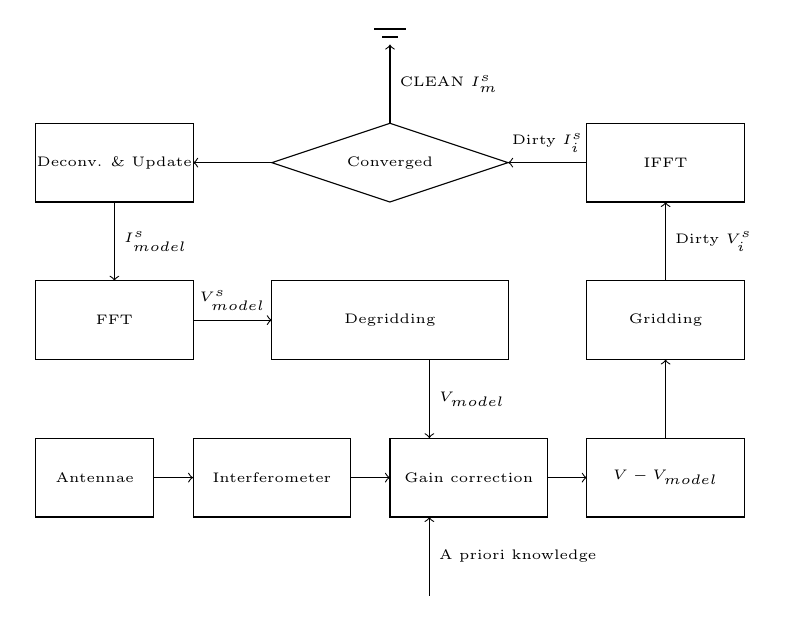
\begin{tikzpicture}[font=\tiny]
    \draw (0,0) rectangle (1.5,1) node at (0.75,0.5) {Antennae};
    \draw[->] (1.5,0.5) -- (2,0.5);
    \draw (2,0) rectangle (4,1) node at (3,0.5) {Interferometer};
    \draw[->] (4,0.5) -- (4.5,0.5);
    \draw (4.5,0) rectangle (6.5,1) node at (5.5,0.5) {Gain correction};
    \draw[->] (6.5,0.5) -- (7,0.5);
    \draw (7,0) rectangle (9,1) node at (8,0.5) {$V - V_{model}$};
    \draw[->] (8,1) -- (8,2);
    \draw (7,2) rectangle (9,3) node at (8,2.5) {Gridding};
    \draw[->] (8,3) -- (8,4) node[pos=.5, right]{Dirty $V_i^s$};
    \draw (7,4) rectangle (9,5) node at (8,4.5) {IFFT};
    \draw[->] (7,4.5) -- (6,4.5) node[pos=.5, above]{Dirty $I_i^s$};
    \draw (3,4.5) -- (4.5,4) -- (6,4.5) -- (4.5,5) -- cycle node at (4.5,4.5) {Converged};
    \draw[->] (3,4.5) -- (2,4.5);
    \draw (0,4) rectangle (2,5) node at (1,4.5) {Deconv. \& Update};
    \draw[->] (1,4) -- (1,3) node[pos=.5, right]{$I_{model}^s$};
    \draw (0,2) rectangle (2,3) node at (1,2.5) {FFT};
    \draw[->] (2,2.5) -- (3,2.5) node[pos=.5, above]{$V_{model}^s$};
    \draw (3,2) rectangle (6,3) node at (4.5,2.5) {Degridding};
    \draw[->] (5,2) -- (5,1) node[pos=.5, right]{$V_{model}$};
    \draw[->] (4.5,5) -- (4.5,6) node[pos=.5, right]{CLEAN $I_m^s$};
    \draw[style=thick] (4.4,6.1) -- (4.6,6.1);
    \draw[style=thick] (4.3,6.2) -- (4.7,6.2);
    \draw[->] (5,-1) -- (5,0) node[pos=.5, right]{A priori knowledge};
 \end{tikzpicture}
 \caption[Imaging pipeline]{The traditional imaging and deconvolution cycle. At the start of the cycle the data is flagged by the observer and known calibration and gain terms are provided.
 An Inverse Fast Fourier Transform is taken after the observed visibilities are uniformly gridded. This dirty sampled image is subsequently deconvolved and the model image updated as per 
 described in the previous section. After this an estimate of the deconvolved visibilities are obtained through an FFT and degridding process, depending on the approach taken. Normally several iterations 
 of this expensive self-calibration cycle is required to converge to a final image of reasonable quality. The directionally dependent effects can be reduced during either gridding 
 or degridding processes for an FFT-based approach. Analytical methods may vary significantly from this illustration.}
 \label{fig_image_cycle}
 \end{mdframed}
 \end{figure}
 
 Exploiting the computational efficiency of the Cooley-Tukey Fast Fourier Transform and its inverse to compute the forward and inverse Discrete Fourier Transforms requires, amongst other considerations, that
 the input is regularly sampled. This sampling is achieved through the process of convolutional gridding. In essense the algorithm can be broken down to four steps as illustrated in figure~\ref{fig_gridding}:
 \begin{enumerate}
  \item The individual complex visibilities are convolved with a highly oversampled function C(u,v). This process spreads them out accross a much wider area in u,v space.
  \item Afterwards the u,v space is regularly sampled.
  \item The image is computed through an Inverse Fast Fourier Transform
  \item A correcting function is applied to the sampled image.
 \end{enumerate}
 \begin{figure}[h]
  \begin{mdframed}
   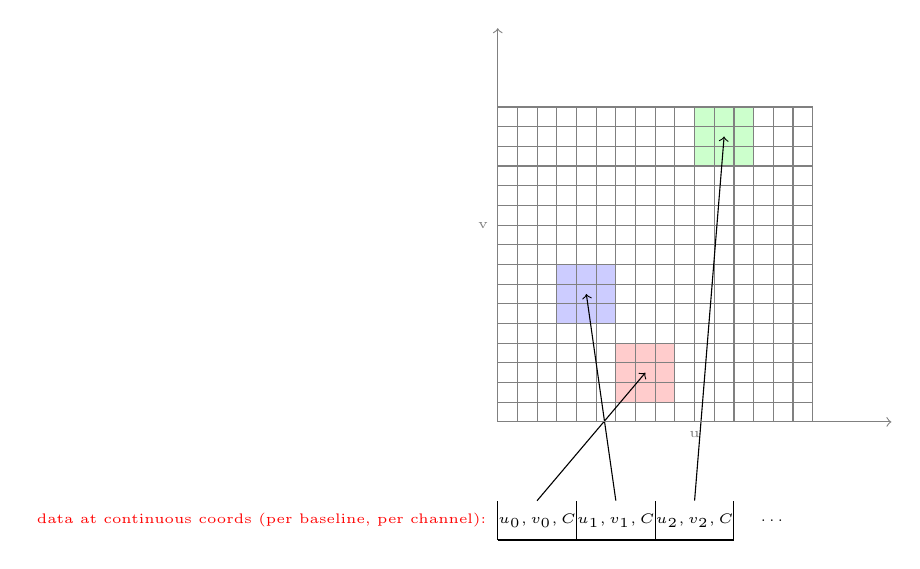
\begin{tikzpicture}[font=\tiny]
    \filldraw[fill=red!20] (4.50,1.75) rectangle (5.25,2.5);
    \filldraw[fill=blue!20] (3.75,2.75) rectangle (4.50,3.50);
    \filldraw[fill=green!20] (5.50,4.75) rectangle (6.25,5.5);
    \draw[step=0.25,gray,thin] (3,1.5) grid (7,5.5);
    \draw[red] node at (0,0.25) {data at continuous coords (per baseline, per channel):};
    \draw node at (6.5,0.25) {\dots};
    \draw[step=1,black] (3,0) grid (6,0.5);
    \draw node at (3.5,0.25) {$u_0,v_0,\mathbb{C}$};
    \draw node at (4.5,0.25) {$u_1,v_1,\mathbb{C}$};
    \draw node at (5.5,0.25) {$u_2,v_2,\mathbb{C}$};
    \draw[->] (3.5,0.5) -- (5-0.125,2.25-0.125);
    \draw[->] (4.5,0.5) -- (4.25-0.125,3.25-0.125);
    \draw[->] (5.5,0.5) -- (6-0.125,5.25-0.125);
    \draw[->,gray] (3,1.5) -- (8,1.5) node[below,pos=0.5]{u};
    \draw[->,gray] (3,1.5) -- (3,6.5) node[left,pos=0.5]{v};
   \end{tikzpicture}
   \caption[Illustration of convolutional gridding]{Each observed visibility (per frequency channel and baseline) is centered at a precomputed coordinate in u,v space and is convolved with 
    some densely sampled function C and binned in a regularly spaced grid. This process essentially spreads each visibility out over a larger area in u,v space. The convolution function is typically sampled
    up to 100 times more regularly than the grid itself \cite{varbanescu2008performance,cornwell2007impact}. It should be clear that this is not the standard convolution as discussed earlier. The fact that the u,v coordinates may vary 
    significantly per baseline may result in two overlapping regions (this poses a problem when parallelizing the algorithm, as will be discussed later on). After all the observed visibilities have been gridded an 
    Inverse Fast Fourier Transform is performed and a correcting function is applied. Each polarization term is typically gridded and transformed to its own, independent, image.}
   \label{fig_gridding}
  \end{mdframed}
 \end{figure}
 Typically the u,v plane is only sparcely sampled as the earth rotates the baselines in u,v space as discussed earlier. This subsampling has the effect of multiplying the observed visibilities with a sampling function. It is also
 not uncommon to find that the u,v space is not uniformly sampled, as pointed out earlier, and that most of the samples are concentrated towards the center of the plane. It is convenient to weigh each sample with its neighbourhood density 
 (the number of visibilities in a neighborhood of grid cells) when sampling sources with both large- and small-scale structure. Natural sampling (typically a weight equal to 1) is used to detect faint sources. After fourier transform
 (by the convolution theorem) the transform of the sampling function is convolved with the image. In image space it is also generally referred to as the Point Spread Function or ``Dirty Beam''. It is possible to remove
 the effects of the Point Spread Function through deconvolution, but deconvolution generally requires a sufficient number of samples to obtain a satisfactory inverse \cite{taylor1999synthesis}.
 
 This sampled observed visibility plane is then convolved with a densely sampled convolution function. The primary goal of this convolution is to interpolate each visibility, but may also limit the aliasing energy outside the support 
 region of the convolving function, as well as limit the interpolation error introduced by using convolutional gridding, instead of the Direct Fourier Transform. Depending on the metrics used to define ``optimal gridding function'' these may vary from a simple truncated sinc or exponential function 
 \cite[Lecture 7]{taylor1999synthesis} to prolate spheriodal functions and approximations to these functions, such as the Keiser Bessel function \cite{jackson1991selection}. Sze Tan \cite{tan1986aperture} derives functions that out-perform prolate spheriodal functions
 on the basis of minimizing aliasing energy, as well as providing an opportunity to trade off the order of interpolation over the area for which the convolution error is small.
 
 It is possible to combine these operations into 
 \begin{equation*}
  I^s_{dirty} = ([I(l,m)*\mathcal{F}^{-1}\{PSF(u,v)\}]\cdot\mathcal{F}^{-1}\{C(u,v)\}) * \mathcal{F}^{-1}\{III(u,v)\}
 \end{equation*}
\section{Narrow field synthesis using the FFT}
\section{Widefield distortions and the problem of non-coplanar baselines}
Evaluating a direct 3D analytical solution over an image cube with n layers soon becomes intractable for large images, specifically in terms of sheer memory requirements for storing these layers. Over a three dimensional cube, M (the number of visibilities),
will be reasonably sparcely sampled, and the number of complex multiplications needed per visibility is estimated to be $\frac{4\lambda B_{max}^3}{D^4}$ \cite{yashar2009tdp}. However, the approach remains embarisingly parallel and can
be scalled over multiple multicore accelerators. A detailed comparison between the throughput achievable by using an analytical approach, compared to convolutional gridding approaches have not been for multicore accelerators \cite{hardy2013direct}.
\section{Non-coplanar facet imaging}
\section{Coplanar facet imaging}
\section{The W-projection algorithm}
\section{Error estimations}
\section{Computational considerations}
\section{Filter precomputation}
\subsection{Anti-aliasing filters}
\subsection{Introducing the W-term}
\subsection{Filter seperability}
\section{Review of previous literature}